\documentclass[11pt,a4paper]{article}

\usepackage[margin=2.4cm]{geometry}
\usepackage{booktabs}
\usepackage{xcolor}
\usepackage{tikz}
\usepackage{amsmath}
\usepackage{enumitem}
\usepackage[colorlinks=true,linkcolor=black,urlcolor=blue]{hyperref}
\usepackage{parskip}
\usetikzlibrary{arrows.meta,positioning}

\definecolor{accent}{HTML}{0A6CA4}
\definecolor{softbg}{HTML}{EEF3F7}
\definecolor{warnbg}{HTML}{FBF2E0}
\definecolor{rule}{HTML}{C9CCD1}

\newcommand{\keyfig}[1]{\textcolor{accent}{\textbf{#1}}}

% \colorbox takes its argument as a single complete group, so it cannot be
% split across an environment boundary. Capture the body in a save box first,
% then colour it once the box is closed.
\newsavebox{\calloutbox}
\newcommand{\calloutcolour}{softbg}
\newenvironment{callout}[1][softbg]
  {\renewcommand{\calloutcolour}{#1}%
   \begin{lrbox}{\calloutbox}%
   \begin{minipage}{\dimexpr\textwidth-2\fboxsep-2\fboxrule\relax}%
   \vspace{2pt}}
  {\vspace{2pt}%
   \end{minipage}%
   \end{lrbox}%
   \begin{center}\colorbox{\calloutcolour}{\usebox{\calloutbox}}\end{center}}

\title{\textbf{Colour to Recipe Prediction for the UFO White PE Ink System}\\[4pt]
       \large Project Report}
\author{Vevo AI Colour Matching, Flint Group}
\date{August 2026}

\begin{document}
\maketitle

\begin{abstract}
\noindent
This report describes a machine learning system that infers an ink formulation
from a measured reflectance spectrum. The system uses a pipeline of two stages:
a multilabel classifier that determines which of fourteen colorants are present,
followed by a regression ensemble that estimates their concentrations. Trained on
2{,}372 production formulas, the system achieves \keyfig{88.2\%} exact set match
on a held out test partition. The report also documents a labelling defect
discovered during review, its correction, the resulting change in measured
accuracy, and the remaining limitations that require laboratory validation
rather than further modelling work.
\end{abstract}

\section{Problem statement}

Matching a customer colour requires a formulator to select colorants and
determine their proportions, then verify the result by drawdown and measurement.
Each iteration consumes ink, substrate and press availability. The objective of
this project is to generate a starting formulation of sufficient quality that
the number of physical iterations is reduced.

The system is positioned as decision support rather than automation. It proposes
a formulation; the formulator retains judgement over whether to accept, adjust or
reject it.

\section{Dataset}

Two files were supplied in CxF format, the ISO standard for colour data exchange.

The primary file contains \keyfig{2{,}372} production formulas from the UFO White
PE system. Each record pairs a \textbf{formulation vector} (the mass fraction of
each of fourteen colorants, constrained to sum to unity) with a \textbf{measured
reflectance spectrum} (36 values sampled at 10\,nm intervals from 380\,nm to
730\,nm, acquired by spectrophotometer in M0 measurement mode). Measurements were
taken over both a light and a dark backing, the latter being informative about
film opacity.

This pairing is what makes supervised learning viable. Each record constitutes a
labelled example of the mapping from formulation to colour, and the inverse
mapping is what the system learns.

A secondary Pantone reference library was used as an independent quality gate.
Formula identifiers encode the Pantone standard each was produced to match, which
permits each measurement to be compared against its intended target. Records
exceeding a colour difference of $\Delta E_{00} = 8$ from their own target were
treated as suspect and excluded, as were records whose colorant fractions failed
to sum to unity within tolerance.

\begin{callout}
\textbf{Partitioning.} The dataset was divided once into a training partition of
2{,}051 records and a held out test partition of \keyfig{297} records. The test
partition was never used for model selection, hyperparameter tuning or threshold
calibration. All figures in this report are measured on that partition.
\end{callout}

\section{Method}

The inference task decomposes naturally into two subproblems of different
character. Identifying \emph{which} colorants are present is a multilabel
classification problem. Estimating \emph{how much} of each is a constrained
regression problem. Treating them separately allows an appropriate method for
each.

\begin{center}
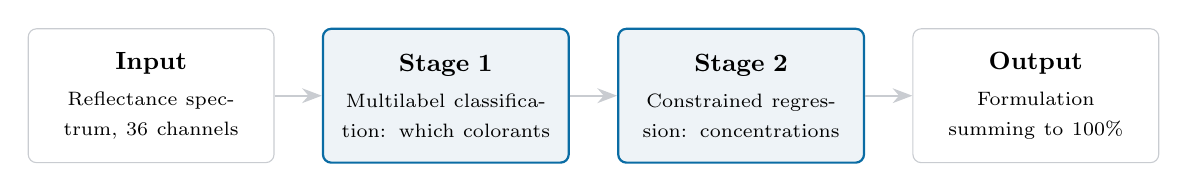
\begin{tikzpicture}[
  node distance=6mm,
  box/.style={draw=rule, rounded corners=3pt, align=center, inner sep=6pt,
              minimum height=17mm, text width=27mm, font=\small},
  hero/.style={box, draw=accent, fill=softbg, thick},
  arr/.style={-{Stealth[length=2.5mm]}, draw=rule, thick}
]
\node[box] (in) {\textbf{Input}\\[2pt]\scriptsize Reflectance spectrum, 36 channels};
\node[hero, right=of in] (s1) {\textbf{Stage 1}\\[2pt]\scriptsize Multilabel classification: which colorants};
\node[hero, right=of s1] (s2) {\textbf{Stage 2}\\[2pt]\scriptsize Constrained regression: concentrations};
\node[box, right=of s2] (out) {\textbf{Output}\\[2pt]\scriptsize Formulation summing to 100\%};
\draw[arr] (in) -- (s1);
\draw[arr] (s1) -- (s2);
\draw[arr] (s2) -- (out);
\end{tikzpicture}
\end{center}

\subsection{Feature representation}

The raw spectrum is augmented with derived features, principally the
Kubelka Munk transform $K/S = (1-R)^2 / 2R$, a standard linearisation of the
relationship between concentration and reflectance, together with first
differences of both the raw and transformed curves to encode curve shape. The
resulting design matrix has 142 columns.

\subsection{Stage 1: colorant identification}

Stage 1 uses \textbf{TabICL}, a pretrained tabular foundation model that performs
in context learning. Rather than fitting fixed parameters during training, the
model attends over the entire training set at inference time and reasons by
analogy with observed examples. It is wrapped in a classifier chain so that each
colorant decision is conditioned on those already made.

TabICL was selected after comparative evaluation against gradient boosting
ensembles, support vector machines, partial least squares discriminant analysis
and TabPFN. It was the strongest performer, and unlike several competitors it
carries a BSD 3 Clause licence permitting commercial use. The principal cost is
inference latency: because the training set is reprocessed on every call,
prediction requires GPU acceleration and takes approximately 60 to 90 seconds.

The reported metric is \textbf{exact set match}, meaning all fourteen presence
decisions must be simultaneously correct for a formula to count as correct. This
is a deliberately strict criterion, since a formulation with one colorant missing
is not usable.

\subsection{Stage 2: concentration estimation}

Given the active colorant set, Stage 2 estimates concentrations. Because colorants
differ substantially in behaviour and in available support, the system performs
per colorant model selection by cross validation across a candidate set including
TabICL regression, a masked softmax neural network and isometric log ratio
regression. The masked softmax architecture enforces the compositional constraint
directly: inactive colorants are assigned negative infinity before the softmax, so
outputs necessarily sum to unity and inactive entries are exactly zero.

\section{A labelling defect and its correction}

\begin{callout}[warnbg]
\textbf{Finding.} The training pipeline applied a presence threshold of
\keyfig{2\%}: any colorant below that mass fraction was labelled absent when
constructing training targets. The laboratory formulates to a minimum of
\keyfig{0.1\%}, a factor of twenty finer.
\end{callout}

The consequence was measured directly. Of 8{,}647 nonzero colorant entries in the
corpus, \keyfig{985} (11.4\%) fell in the affected band, distributed across
\keyfig{777} of 2{,}372 formulas (32.8\%). Approximately one third of the training
corpus was therefore presented to the model with at least one ingredient removed.

The threshold also fell within a dense region of the concentration distribution.
467 entries lie within 0.5 percentage points of the boundary, split almost evenly
either side. Consequently, near identical formulations differing by hundredths of
a percentage point received opposite labels, injecting irreducible noise into the
training targets.

The system was retrained with the threshold set to the laboratory working minimum.
Because the two configurations score different labelling conventions, they are not
directly comparable; both models were therefore evaluated against both label
definitions on the identical test partition.

\begin{table}[h]
\centering
\begin{tabular}{lrr}
\toprule
Model & vs.\ 2\% labels & vs.\ 0.1\% labels \\
\midrule
Incumbent, trained at 2\%   & 86.53\% & \textbf{59.26\%} \\
Retrained at 0.1\%          & 61.95\% & \textbf{88.22\%} \\
\bottomrule
\end{tabular}
\caption{Exact set match, 297 held out formulas. Each model performs well on the
labelling convention it was trained for. The operationally relevant comparison is
the right hand column.}
\end{table}

\begin{callout}
\textbf{Interpretation.} A ceiling argument bounds the comparison. Only 197 of the
297 test formulas carry an identical active set under both conventions, so an
incumbent model performing perfectly at its own task could not exceed
\keyfig{66.33\%} against 0.1\% labels. The previously reported figure of 86.53\%
was measured against a coarser criterion than laboratory practice and should not
be presented as a baseline for the current system.
\end{callout}

Counter to expectation, accuracy \emph{increased} despite the task becoming
strictly harder (mean active colorants per formula rose from 3.25 to 3.67, and
positive decisions increased by 13\%). The explanation is the removal of
contradictory targets described above: label noise was reduced by more than
task difficulty was increased.

\section{Results}

\begin{table}[h]
\centering
\begin{tabular}{lrl}
\toprule
Metric & Value & Interpretation \\
\midrule
Exact set match          & 88.22\% & All fourteen decisions simultaneously correct \\
Per decision accuracy    & 98.87\% & Over 4{,}158 binary decisions \\
Macro F1                 & 0.936   & Averaged across colorants \\
Stage 2 MAE              & 0.0090  & 0.90 percentage points on active cells \\
Within tolerance         & 41\%    & Formulas estimated inside $\Delta E_{00} < 1$ \\
\bottomrule
\end{tabular}
\caption{Performance on the held out partition.}
\end{table}

Relative to a nearest neighbour baseline, in which the recipe of the closest
existing shade is copied, the system produces formulations approximately
\keyfig{three times} closer in colour terms and an order of magnitude closer in
composition.

The system is deployed as a local web application. It additionally raises review
flags for formulations containing Red 032, and for those exceeding the standard
formulation rule of at most three chromatic colorants plus transparent white.

\section{Limitations}

\begin{callout}[warnbg]
\textbf{No formulation produced by this system has been physically drawn down and
measured.} All reported figures quantify agreement between predicted and recorded
formulations. They are measures of formulation accuracy, not colour accuracy, and
must not be presented as the latter.
\end{callout}

\begin{enumerate}[leftmargin=*,itemsep=4pt]

\item \textbf{Concentration estimation is the binding constraint.} Colorant
identification is largely solved. The residual concentration error translates to
an estimated colour difference in the region of 1.5 to 3 $\Delta E_{00}$, against
a customer acceptance criterion of 1.0. This estimate derives from direction
matched comparisons among real formula pairs and carries meaningful uncertainty.

\item \textbf{Red 032 is inadequately supported.} It appears in 31 training
formulas. Six distinct modelling strategies have been evaluated without success.
This is a data scarcity constraint, not an algorithmic one.

\item \textbf{The corpus exhibits intrinsic variability.} Formulations differing
by hundredths of a percentage point measure approximately 1 $\Delta E_{00}$
apart, indicating that factors outside the formulation, plausibly film weight,
substrate lot or press conditions, materially affect the outcome. No model can
recover from a formulation what the formulation does not determine.

\item \textbf{Transparent white is underdetermined by colour.} It is
approximately 3.81 times less identifiable from spectral data than other
colorants, consistent with laboratory practice in which the transparent white
level is set by shade after the chromatic formulation is finalised.

\end{enumerate}

\section{Recommendations}

Algorithmic avenues have been substantially exhausted. Kernel and Gaussian
process methods were evaluated across all fourteen colorants and none met the
adoption criterion. Joint mode decoding was bounded analytically and shown to be
incapable of exceeding 89.90\%. Commercially licensed alternative models were
surveyed and found either to prohibit commercial use or to rank below the
incumbent. Remaining gains therefore require laboratory data.

\begin{enumerate}[leftmargin=*,itemsep=6pt]

\item \textbf{Replicate measurements, obtainable only during the forthcoming
trial.} Prepare and measure the same formulation three or four times, across
several shades. The corpus contains no replicates, so process repeatability
cannot presently be separated from model error. This determines whether a
$\Delta E_{00} < 1$ criterion is attainable in principle or whether the system
should be positioned as proposing formulations for human confirmation.

\item \textbf{Additional samples for four colorants:} Red 032, Blue 072, Purple
and Rhodamine Red. On shades containing Blue 072 the system errs in approximately
45\% of cases, and on Red 032 in approximately one third. These colorants are
rare corpus wide, so the effect on aggregate accuracy is limited, but the effect
on individual jobs requiring them is substantial.

\item \textbf{A baseline for comparison.} The typical first attempt accuracy of an
experienced formulator is not known. Without it, the time saving attributable to
the system cannot be quantified.

\end{enumerate}

\vspace{6pt}
\hrule
\vspace{6pt}
\footnotesize
\noindent
All figures measured on 297 formulas held out from training and excluded from
model selection. Accuracy denotes agreement between predicted and recorded
formulations. Colour accuracy awaits physical validation.

\end{document}
